\subsection{Speech Components}
\label{sec:speech-components}

Our interaction roadmap begins with speech components, which bridge speech signals and model representations to support perception and generation. Speech can be represented either as discrete units obtained through encoding and quantization or as sequences of continuous vectors, giving rise to discrete and continuous speech representations, respectively. Across both representation types, we examine how component designs preserve speech information, support downstream modeling, and manage computational cost. For discrete representations, we review tokenization designs that emphasize semantic content, acoustic detail, or their combination; for continuous representations, we examine the encoding and decoding interfaces that connect speech with language models. Figure~\ref{fig:speech-components} provides an overview of discrete and continuous speech representations and their associated components. Table~\ref{tab:speech-components} summarizes representative speech components and systems, highlighting their representations and key design choices.

\begin{figure}[htbp]
    \centering
    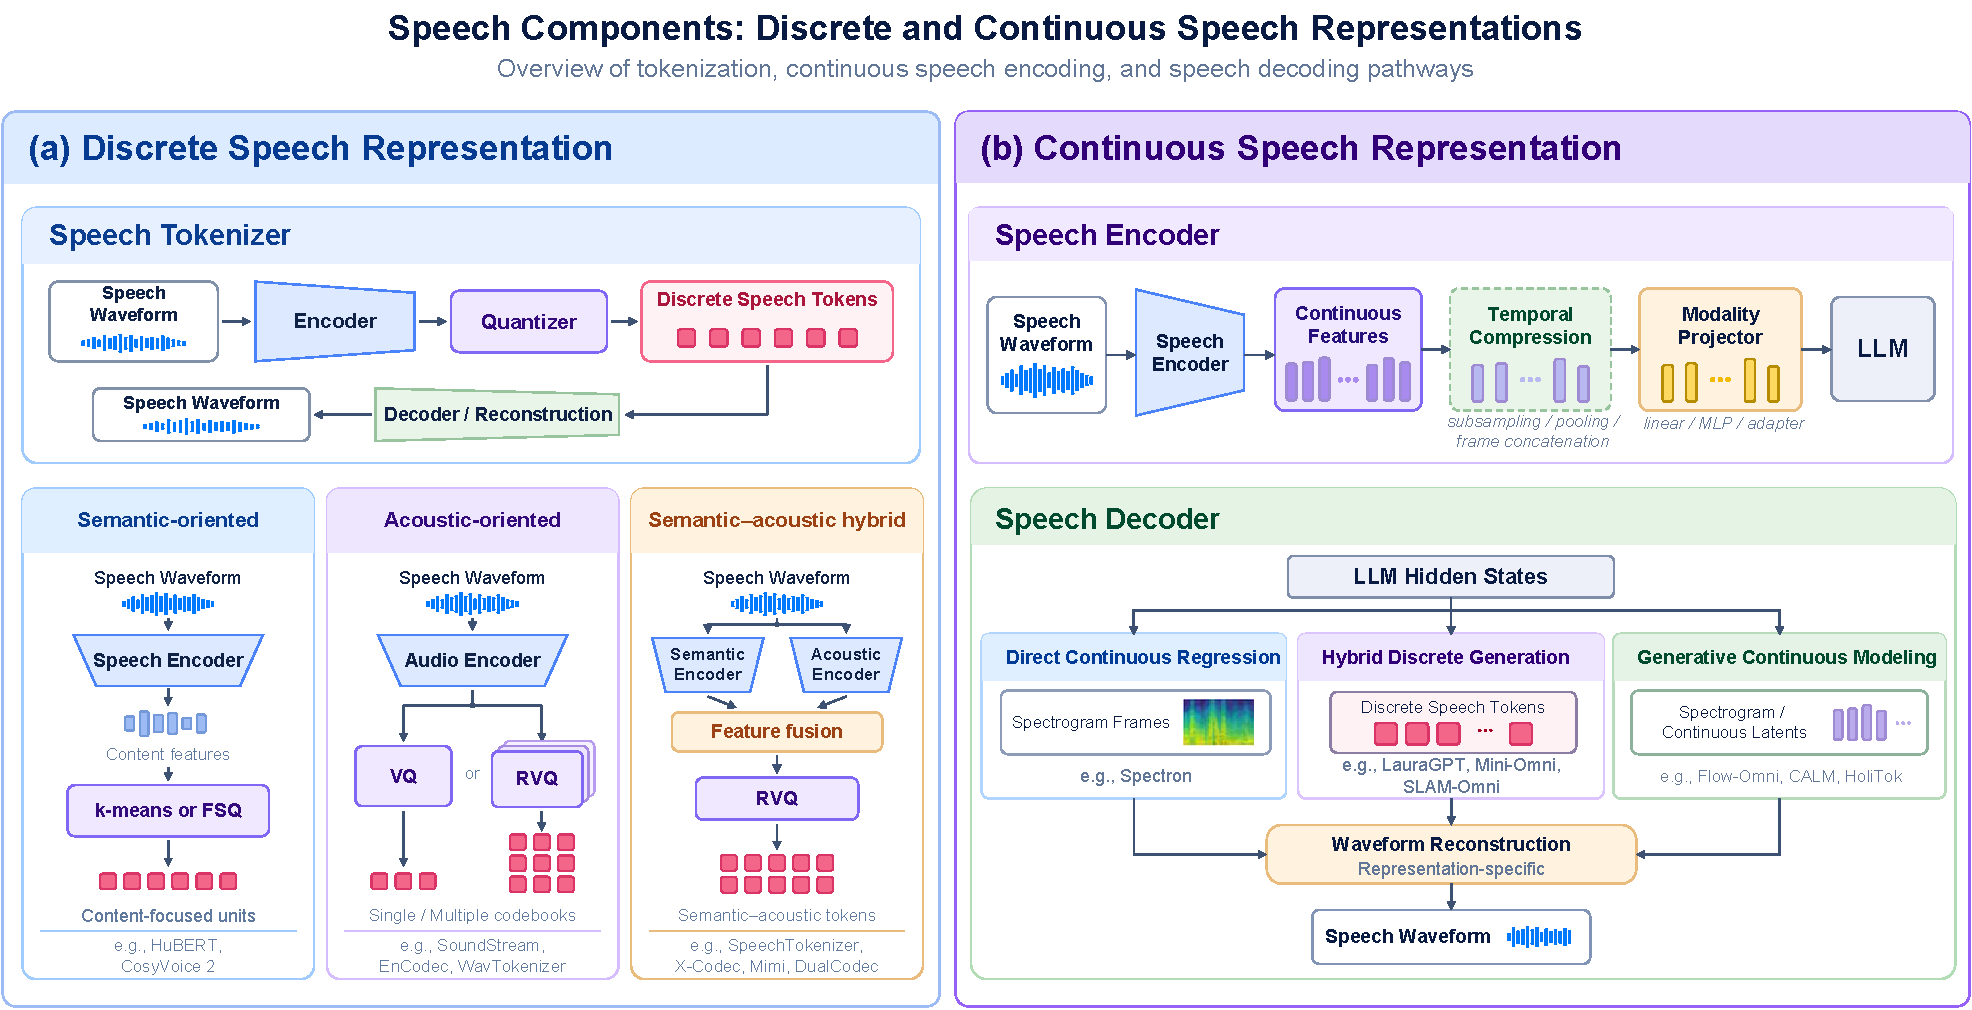
\includegraphics[width=\textwidth]{figures/speech_components.pdf}
    \caption{Overview of speech components for discrete and continuous speech representations. (a) Discrete speech tokenization with semantic-oriented, acoustic-oriented, and semantic--acoustic hybrid designs. (b) Continuous speech representation, comprising speech encoding (top) and speech decoding (bottom). The encoder pathway combines feature extraction, optional temporal compression, and modality projection; the decoder pathways include direct continuous regression, hybrid discrete generation, and generative continuous modeling. The hybrid pathway combines continuous speech input with discrete output tokens.}
    \label{fig:speech-components}
\end{figure}

\subsubsection{Discrete Speech Representation}
\label{sec:discrete-speech-representation}

Discrete speech representations are obtained by encoding and quantizing speech waveforms into sequences of discrete tokens drawn from a finite vocabulary. This enables speech models to adopt the autoregressive modeling and training mechanisms used in large language models (LLMs). The resulting tokens can be converted back into speech through a suitable decoding module~\citep{DBLP:conf/acl/CuiYJMZWGK25}. The core design trade-offs concern sequence length, linguistic content preservation, and acoustic fidelity~\citep{DBLP:journals/pami/GuoLWLSZDCLY26,DBLP:journals/tmlr/MousaviMMPSWYKPMRELLSWK25}. Based on their relative emphasis on linguistic content and acoustic reconstruction, we group existing methods into three broad categories: semantic-oriented, acoustic-oriented, and semantic--acoustic hybrid approaches, as illustrated in Figure~\ref{fig:speech-components}(a)~\citep{DBLP:conf/acl/CuiYJMZWGK25,DBLP:journals/pami/GuoLWLSZDCLY26}.

\textbf{Semantic-oriented.} These methods prioritize linguistic content, typically extracting features from self-supervised or speech recognition models and converting them into discrete units through clustering or quantization. HuBERT learns representations by predicting cluster-based pseudo-labels at masked positions; its hidden features can subsequently be clustered using k-means to obtain content-related speech tokens~\citep{DBLP:journals/taslp/HsuBTLSM21}. CosyVoice 2 incorporates finite scalar quantization (FSQ) into its speech recognition encoder: recognition supervision encourages content preservation, whereas FSQ improves codebook utilization~\citep{DBLP:journals/corr/abs-2412-10117}. These units support downstream content modeling and can reduce sequence length when combined with temporal compression. However, they do not guarantee the preservation of fine acoustic detail; waveform generation commonly relies on additional acoustic modeling or reference conditioning to supply timbre and prosody~\citep{DBLP:journals/pami/GuoLWLSZDCLY26,DBLP:journals/corr/abs-2412-10117}.

\textbf{Acoustic-oriented.} These methods prioritize reconstruction quality and typically adopt an encoder--quantizer--decoder architecture. SoundStream and EnCodec use residual vector quantization (RVQ) to progressively encode residual information in latent features, combining reconstruction and adversarial objectives to preserve acoustic detail~\citep{DBLP:journals/taslp/ZeghidourLOST22,DBLP:journals/tmlr/DefossezCSA23}. WavTokenizer explores a single-codebook alternative, improving the quantization space and decoder to reduce the number of discrete indices while maintaining reconstruction quality~\citep{DBLP:conf/iclr/Ji00C0Z0C0LZY0J25}. This favors high-fidelity synthesis, but reconstruction quality does not ensure that linguistic content is readily modeled. Multi-codebook designs also increase the number of indices per frame and, when serialized, the sequence length, requiring downstream models to balance acoustic fidelity against prediction cost~\citep{DBLP:conf/iclr/ZhangZLZQ24,DBLP:conf/aaai/YeSL00DKCPLGX25,DBLP:journals/corr/abs-2410-00037}.

\textbf{Semantic--acoustic hybrid.} These methods combine semantic supervision with acoustic reconstruction to balance content preservation and acoustic fidelity. SpeechTokenizer distills HuBERT representations into the first RVQ layer, encouraging it to capture linguistic content while subsequent layers encode additional acoustic detail~\citep{DBLP:conf/iclr/ZhangZLZQ24}. X-Codec fuses semantic and acoustic features before quantization and introduces a semantic reconstruction loss~\citep{DBLP:conf/aaai/YeSL00DKCPLGX25}. Mimi organizes semantic vector quantization and acoustic RVQ in parallel, combining low-frame-rate representations with causal encoding and decoding for streaming operation~\citep{DBLP:journals/corr/abs-2410-00037}. DualCodec uses separate speech-representation and waveform encoding streams, enriching the first codec layer with content-related information while the remaining layers encode residual acoustic information~\citep{DBLP:conf/interspeech/LiLLHWWZ025}. These designs provide a shared interface for content modeling and speech generation, but must allocate finite representation capacity between linguistic and acoustic information. A lower frame rate does not necessarily reduce the total prediction workload: codebook count and generation factorization also matter. Likewise, layer-wise specialization should not be interpreted as complete information disentanglement~\citep{DBLP:conf/iclr/ZhangZLZQ24,DBLP:journals/corr/abs-2410-00037,DBLP:conf/interspeech/LiLLHWWZ025}.

Together, these approaches offer different trade-offs among linguistic content, acoustic detail, and modeling cost. For real-time interaction, their suitability depends jointly on token frame rate, codebook count, generation factorization, causality, and look-ahead requirements, rather than compression ratio or offline reconstruction quality alone~\citep{DBLP:journals/taslp/ZeghidourLOST22,DBLP:journals/corr/abs-2410-00037}.


\subsubsection{Continuous Speech Representation}
\label{sec:continuous-speech-representation}

Continuous speech representations model speech as sequences of real-valued vectors rather than indices from a finite codebook. Avoiding explicit quantization can help preserve fine-grained semantic, prosodic, timbral, and other paralinguistic information~\citep{DBLP:journals/corr/abs-2310-04673,DBLP:conf/naacl/LiXSCK25}. Their integration with text-based LLMs nevertheless requires adaptations to representation alignment and, when continuous values are predicted, to the output and sampling mechanisms. Sequence compression, cross-modal alignment, and continuous-space generation therefore constitute central design challenges~\citep{DBLP:conf/emnlp/AlgayresANCSSD23,DBLP:conf/iclr/NachmaniLHSAMRS24,DBLP:journals/corr/abs-2310-04673,DBLP:journals/corr/abs-2412-04917}.

Early work such as tGSLM demonstrated language modeling with continuous speech embeddings, using a learnable Lexical Embedder, contrastive loss, and k-nearest-neighbor (k-NN) sampling~\citep{DBLP:conf/emnlp/AlgayresANCSSD23}. When continuous representations are integrated with pretrained LLMs, these modeling questions extend to two component interfaces: speech encoders provide continuous input representations, while speech decoders convert model outputs into speech.

\paragraph{Speech Encoder}
\label{sec:speech-encoder}

A typical continuous input pathway combines speech feature extraction, temporal compression, and modality projection, as shown in Figure~\ref{fig:speech-components}(b). The speech encoder extracts continuous acoustic and semantic features; subsampling, pooling, or frame concatenation can reduce their sequence length before a linear projection or multilayer perceptron (MLP) adapter maps them into the LLM embedding space. Temporal compression limits the computational cost of high-frame-rate inputs, while modality projection enables the language model to process speech representations~\citep{DBLP:conf/iclr/NachmaniLHSAMRS24,DBLP:journals/corr/abs-2408-16725,DBLP:conf/acl/Chen0YLLXN00L0025}.

Spectron follows a direct implementation of this interface: a pretrained speech encoder produces continuous features, and a projection layer maps them into the language model's embedding space without first converting them into discrete speech tokens~\citep{DBLP:conf/iclr/NachmaniLHSAMRS24}. LauraGPT, Mini-Omni, and SLAM-Omni follow a similar encoder--adapter interface, extracting continuous speech features with a Conformer (LauraGPT) or Whisper encoder (Mini-Omni and SLAM-Omni) and mapping them into the language model's embedding space through adapters or projection layers~\citep{DBLP:journals/corr/abs-2310-04673,DBLP:journals/corr/abs-2408-16725,DBLP:conf/acl/Chen0YLLXN00L0025}. Across these designs, the main interface challenge is to preserve useful speech information while controlling sequence length and aligning the resulting features with the language model.

\paragraph{Speech Decoder}
\label{sec:speech-decoder}

Speech generation maps language model states to acoustic representations and ultimately to waveforms. The speech decoder pathways in Figure~\ref{fig:speech-components}(b) include direct continuous regression, hybrid discrete generation, and generative continuous modeling. In direct continuous regression, Spectron generates text before autoregressively predicting spectrogram frames, which a vocoder converts into a waveform~\citep{DBLP:conf/iclr/NachmaniLHSAMRS24}. Although this approach avoids codec quantization, frame-level generation results in long acoustic sequences and substantial computational overhead. Moreover, the sequential generation of text and spectrogram frames poses challenges for streaming generation. Continuous input representations can also be paired with discrete output tokens, as in the hybrid discrete generation approaches adopted by LauraGPT, Mini-Omni, and SLAM-Omni~\citep{DBLP:journals/corr/abs-2310-04673,DBLP:journals/corr/abs-2408-16725,DBLP:conf/acl/Chen0YLLXN00L0025}. Their speech encoders produce continuous speech representations, while their generation modules autoregressively predict discrete speech tokens, such as codec or semantic tokens.

In generative continuous modeling, Flow-Omni combines a pretrained autoregressive LLM with a lightweight generation module trained using flow matching~\citep{DBLP:journals/corr/abs-2412-04917}. Conditioned on language model states, the module models a distribution over continuous acoustic representations instead of directly regressing a single target frame. CALM uses continuous latents from an audio variational autoencoder (VAE), with a Transformer providing contextual representations that condition a consistency-based generation module~\citep{DBLP:conf/iclr/RouardORZD26}. Related work also explores the continuous representations used for speech generation: Cont-SPT develops a continuous speech tokenizer for text-to-speech (TTS)~\citep{DBLP:conf/naacl/LiXSCK25}, while HoliTok explores a shared continuous latent space for speech understanding and generation~\citep{DBLP:journals/corr/abs-2605-29948}.

Together, the encoder and decoder interfaces connect continuous speech representations to perception and generation. Encoders extract, compress, and align speech features for the language model, while decoders generate speech from model outputs. The design of these interfaces influences how information preserved from the input is reflected in response content and acoustic expression.

\begin{TakeawayBox}{Takeaways: Speech Components}

Discrete speech representations offer complementary trade-offs: semantic-oriented units emphasize content, acoustic-oriented codes emphasize reconstruction, and hybrid designs combine both under representation and prediction constraints. Continuous representations avoid explicit quantization but require suitable alignment and continuous-output modeling. Across both approaches, information preservation must be evaluated together with sequence structure and downstream computation.
\end{TakeawayBox}

\begin{table*}[!htbp]
    \centering
    \caption{Overview of speech component methods and representative systems.
    RVQ: residual vector quantization; FSQ: finite scalar quantization;
    VAE: variational autoencoder.}
    \label{tab:speech-components}
    \footnotesize
    \setlength{\tabcolsep}{3pt}
    \renewcommand{\arraystretch}{1.0}
    \setlength{\defaultaddspace}{2pt}
    \begin{tabular}{@{}
        >{\raggedright\arraybackslash}p{\dimexpr0.18\linewidth-6pt\relax}
        >{\raggedright\arraybackslash}p{\dimexpr0.14\linewidth-6pt\relax}
        >{\raggedright\arraybackslash}p{\dimexpr0.28\linewidth-6pt\relax}
        >{\raggedright\arraybackslash}p{\dimexpr0.40\linewidth-6pt\relax}@{}}
        \toprule
        \textbf{Representation} & \textbf{Component} & \textbf{Work} & \textbf{Highlight} \\
        \midrule
        Discrete & Semantic tokenizer & HuBERT~\citep{DBLP:journals/taslp/HsuBTLSM21} &
        Content-related units support linguistic modeling; reconstruction needs an additional decoder. \\
        \addlinespace
        Discrete & Semantic tokenizer & CosyVoice 2~\citep{DBLP:journals/corr/abs-2412-10117} &
        Recognition supervision preserves content; FSQ improves utilization; synthesis uses acoustic conditioning. \\
        \addlinespace
        Discrete & Acoustic tokenizer & SoundStream~\citep{DBLP:journals/taslp/ZeghidourLOST22}; EnCodec~\citep{DBLP:journals/tmlr/DefossezCSA23} &
        RVQ preserves acoustic detail but increases the number of per-frame prediction targets. \\
        \addlinespace
        Discrete & Acoustic tokenizer & WavTokenizer~\citep{DBLP:conf/iclr/Ji00C0Z0C0LZY0J25} &
        Single-codebook compression reduces prediction targets while prioritizing reconstruction quality. \\
        \addlinespace
        Discrete & Semantic--\newline acoustic\newline hybrid tokenizer & SpeechTokenizer~\citep{DBLP:conf/iclr/ZhangZLZQ24} &
        First-layer distillation emphasizes content; later RVQ layers supply acoustic detail. \\
        \addlinespace
        Discrete & Semantic--\newline acoustic\newline hybrid tokenizer & X-Codec~\citep{DBLP:conf/aaai/YeSL00DKCPLGX25} &
        Joint quantization and semantic reconstruction combine content cues with acoustic fidelity. \\
        \addlinespace
        Discrete & Semantic--\newline acoustic\newline hybrid tokenizer & Mimi~\citep{DBLP:journals/corr/abs-2410-00037} &
        Causal, low-frame-rate coding supports streaming; multiple codebooks retain prediction overhead. \\
        \addlinespace
        Discrete & Semantic--\newline acoustic\newline hybrid tokenizer & DualCodec~\citep{DBLP:conf/interspeech/LiLLHWWZ025} &
        Dual encoding enriches first-layer content; low frame rate shortens temporal sequences. \\
        \midrule
        Continuous & Embedding model & tGSLM~\citep{DBLP:conf/emnlp/AlgayresANCSSD23} &
        Word-sized embeddings, contrastive training, and nearest-neighbor sampling. \\
        \addlinespace
        Continuous & Encoder; decoder & Spectron~\citep{DBLP:conf/iclr/NachmaniLHSAMRS24} &
        Projects speech features into the LLM; predicts spectrogram frames after text. \\
        \addlinespace
        Continuous input;\newline discrete output & Encoder; decoder & LauraGPT~\citep{DBLP:journals/corr/abs-2310-04673} &
        Conformer input features with discrete codec-code generation. \\
        \addlinespace
        Continuous input;\newline discrete output & Encoder; decoder & Mini-Omni~\citep{DBLP:journals/corr/abs-2408-16725} &
        Whisper encoder and audio adapter with discrete audio-token generation. \\
        \addlinespace
        Continuous input;\newline discrete output & Encoder; decoder & SLAM-Omni~\citep{DBLP:conf/acl/Chen0YLLXN00L0025} &
        Downsampled Whisper features and linear projection; semantic-token output. \\
        \addlinespace
        Continuous output & Generation module & Flow-Omni~\citep{DBLP:journals/corr/abs-2412-04917} &
        LLM states condition flow matching over acoustic representations. \\
        \addlinespace
        Continuous & Tokenizer & Cont-SPT~\citep{DBLP:conf/naacl/LiXSCK25} &
        Continuous speech vectors avoid discrete quantization for TTS. \\
        \addlinespace
        Continuous & Latent model; generator & CALM~\citep{DBLP:conf/iclr/RouardORZD26} &
        Audio VAE latents with context-conditioned, consistency-based generation. \\
        \addlinespace
        Continuous & Shared tokenizer & HoliTok~\citep{DBLP:journals/corr/abs-2605-29948} &
        Compact shared latents support both speech understanding and generation. \\
        \bottomrule
    \end{tabular}
\end{table*}

